\documentclass{article}
\usepackage{graphicx} % Required for inserting images
\usepackage[spanish]{babel}
\usepackage{booktabs}
\usepackage{adjustbox}
\usepackage{amsmath}
\usepackage{amssymb}

\title{Emisión de $CO_2$ de vehículos que circulan en México en base a sus características}
\author{Luis Felipe Rangel Salazar}
\date{Julio 2024}

\begin{document}

\maketitle

\section{Introducción}

El conjunto de datos con el que se va a trabajar representa un listado de distintos vehículos que circulan en México junto con sus características.

El objetivo del trabajo es identificar las principales características de un vehículo que afectan en su cantidad de emisiones de $CO_2$.

Se pretende hacer un análisis predictivo del nivel de contaminante que emiten los vehículos en base a algunas de sus características, y por consecuencia en la cantidad de dióxido de carbono ($CO_2$) que emiten, aplicando algunos métodos de Aprendizaje Supervisado o No Supervisado.



\section{Descripción de los datos}

La base de datos consta de 4,601 registros con 19 variables originalmente.

\begin{itemize}
    \item CO2 (g/km) [variable objetivo]
    \item Marca
    \item Submarca
    \item Versión
    \item Modelo
    \item Trans.
    \item Comb.
    \item Cilindros
    \item Categoría
    \item R. Ciudad (km/l)
    \item R. Carr. (km/l)
    \item R. Comb. (km/l)
    \item R. Ajust. (km/l)
    \item Nox (g/1000km)
    \item Calificación Gas Ef. Inv.
    \item Calificación Contam. Aire
    \item Tamaño (L)
    \item Potencia (HP)
    \item Hibrido 
\end{itemize}

\subsection{Selección de variables}

Las siguientes variables fueron descartadas:

\begin{itemize}
    \item R. Comb. (km/l)
    \item R. Ajust. (km/l)
    \item Nox (g/1000km)
    \item Calificación Gas Ef. Inv.
    \item Calificación Contam. Aire
    \item Versión
    \item Comb.
\end{itemize}

Esto, debido a que estas variables se derivan o se calculan en base a otras que ya estamos considerando, tales como R. Ciudad (km/l) y R. Carr. (km/l), con lo que si las incluimos tendríamos un problema de colinealidad. En el caso de Nox (g/1000km) y Comb. se excluyen por tener un bajo estadístico F en relación al CO2 (g/km). La variable Versión también debe ser excluida debido a que hay muchas categorías de Versión (3,118 etiquetas de 4,601 registros), esta variable no permite un análisis al casi tener cada vehículo su propia Versión.

Con esto se corre el riesgo de tener overfitting y por lo tanto la sugerencia es remover este campo.


\subsection{Estadística descriptiva básica}



\newpage

\begin{figure}[h]
  \centering
  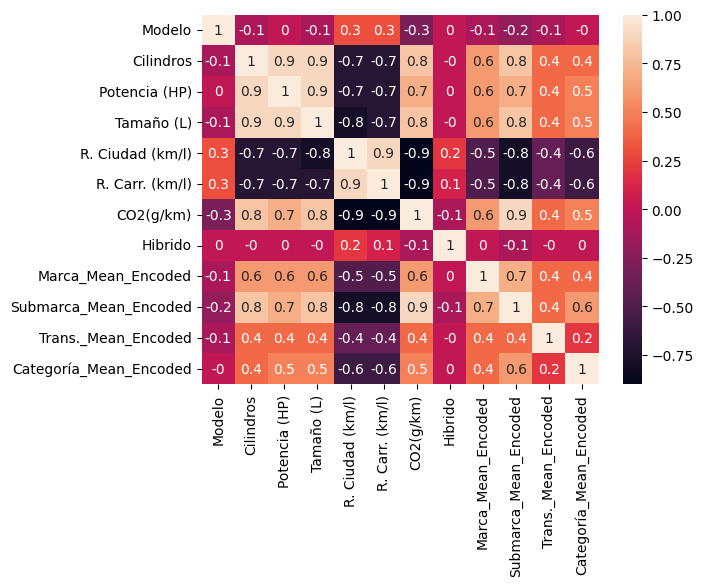
\includegraphics[width=1\linewidth]{imagenes/1_correlations.png}
  \caption{Matriz de correlaciones}
  \label{fig:figura1}
\end{figure}

Como se puede ver en la figura \ref{fig:figura1}, las variables de Cilindros, Potencia y Tamaño son las que se encuentran más correlacionadas positivamente entre ellas. De igual forma, la variable Submarca tiene una correalación positiva alta con la variable respuesta $CO_2$. Las variables de Rendimiento en Ciudad y Rendimiento en Carretera son las que presentan mayor correlación negativa con la variable respuesta $CO_2$.

En los cuadros \ref{table:tabla1} y \ref{table:tabla2} se muestran las principales estadísticas descriptivas de cada variable.

\begin{table}[ht]
    \begin{adjustbox}{max width=1\textwidth}
        \begin{tabular}{lrrrrr}
        \toprule
         & Modelo & Cilindros & Potencia (HP) & Tamaño (L)\\
        \midrule
        Conteo & 4601 & 4601 & 4601 & 4601\\
        Media & 2014.18 & 5.33 & 255.29 & 2.87\\
        Desviación & 2.16 & 1.8 & 132.920000 & 1.350000\\
        Min & 2011 & 3 & 60 & 0.9\\
        25\% & 2012 & 4 & 150 & 1.8\\
        50\% & 2014 & 4 & 220 & 2.5\\
        75\% & 2016 & 6 & 330 & 3.6\\
        Max & 2018 & 12 & 888 & 8.4\\
        \bottomrule
        \end{tabular}
    \end{adjustbox}
    \centering
    \caption{Estadística descriptiva 1}
    \label{table:tabla1}
\end{table}

\begin{table}[ht]
    \begin{adjustbox}{max width=1\textwidth}
        \begin{tabular}{lrrrr}
        \toprule
         & R. Ciudad (km/l) & R. Carr. (km/l) & CO2(g/km) & Hibrido \\
        \midrule
        Conteo & 4601 & 4601 & 4601 & 4601 \\
        Media & 10.6 & 16.6 & 256.73 & 0.01 \\
        Desviación & 3.29 & 4.19 & 75.63 & 0.1 \\
        Min & 3.1 & 6.7 & 107 & 0 \\
        25\% & 8.2 & 13.44 & 200 & 0 \\
        50\% & 10.42 & 16.39 & 244 & 0 \\
        75\% & 12.82 & 19.6 & 299 & 0 \\
        Max & 27.46 & 31.3 & 627 & 1 \\
        \bottomrule
        \end{tabular}
    \end{adjustbox}
    \centering
    \caption{Estadística descriptiva 2}
    \label{table:tabla2}
\end{table}

\newpage

\section{Preprocesamiento}

Se generó el campo Hibrido con un 1 si el vehículo es híbrido y 0 si no lo es, en base a la descripción del vehículo que se podía extraer de los campos Versión y Submarca. Se eliminaron los registros con valores nulos y se redefinieron las variables categóricas usando el método de Mean Encoding.


\section{Agrupamiento}

Se realizó un agrupamiento para la variable Submarca con $CO_2$ por el método de K-Medias.

Primero se obtuvo que la cantidad de grupos adecuada era $K=4$ de acuerdo al gráfico de codo \ref{fig:figura2}.

\begin{figure}[h]
  \centering
  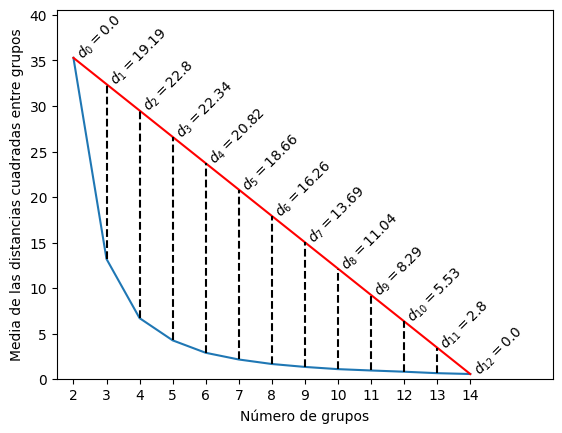
\includegraphics[width=.7\linewidth]{imagenes/2_codo.png}
  \caption{Gráfica de codo}
  \label{fig:figura2}
\end{figure}

\newpage

El resultado de emplear K-medias para agrupar las submarcas se puede apreciar en la figura \ref{fig:figura3}.

\begin{figure}[h]
  \centering
  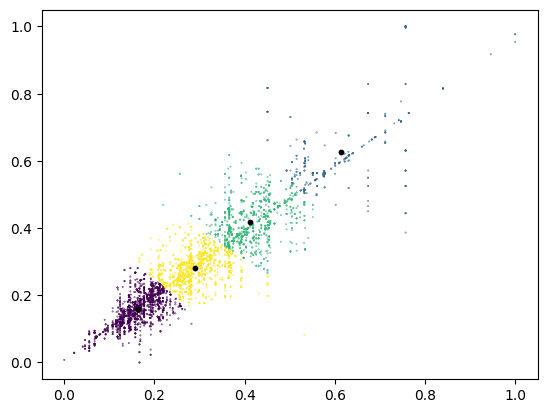
\includegraphics[width=.65\linewidth]{imagenes/3_k-medias.png}
  \caption{Gráfica de codo}
  \label{fig:figura3}
\end{figure}


\newpage

\subsection{Metodología de agrupamiento}

    \textbf{$K$-medias}\n

    Esta técnica no supervisada consiste en generar $K \in \mathbb{N}$ grupos para $n$ elementos que incluyan a los $n_k$ más cercanos (con base en cierta medida de distancia, generalmente euclidiana) respecto a un centroide $c_k = (\hat{x}, \hat{y})$ tal que\n,
    $$\hat{x} = \frac{1}{n_k} \sum_{i \in K} x_i$$ \n
    $$\hat{y} = \frac{1}{n_k} \sum_{i \in K} y_i$$ \n
    \n
    Formalmente, la distancia más cercana respecto a los centroides $c_k$ se define como la minimización del error cuadrado para cada grupo\n,
    $$\text{SS}_k = \sum_{i \in K} (x_i - \hat{x}_k)^2 + (y_i - \hat{y}_k)^2.$$\n

    Este algoritmo es iterativo y tiene como función objetivo\n,

    $$\min \sum_{i \in K} \text{SS}_k$$


\section{Regresión Lineal}

Se aplica el método supervisado de Regresión Lineal para pronosticar emisiones de CO2 en base al resto de las variables seleccionadas y se calculan al final métricas para analizar los errores.

El resultado fue la siguiente ecuación:

\begin{multline*}
y = 0.3408 + X_0 (-0.0193) + X_1 (0.0887) + X_2 (-0.0788) + X_3 (0.091) \\
+ X_4 (-0.244) + X_5 (-0.2569) + X_6 (-0.0117) + X_7 (0.0334) \\
+ X_8 (0.372) + X_9 (0.017) + X_{10} (-0.0277)
\end{multline*}

donde, 

\begin{itemize}
    \item $X_0$: Modelo
    \item $X_1$: Cilindros
    \item $X_2$: Potencia (HP)
    \item $X_3$: Tamaño (L)
    \item $X_4$: R. Ciudad (km/l)
    \item $X_5$: R. Carr. (km/l)
    \item $X_6$: Hibrido
    \item $X_7$: Marca\_Mean\_Encoded
    \item $X_8$: Submarca\_Mean\_Encoded
    \item $X_9$: Trans.\_Mean\_Encoded
    \item $X_{10}$: Categoría\_Mean\_Encoded
\end{itemize}


\subsection{Metodología de regresión lineal}

En una regresión se busca ajustar una curva a los datos minimizando el error. La regresión más sencilla es la regresión lineal donde se pretende predecir valores $Y$ a partir de determinados $n$ variables $X$ mediante la ecuación lineal $Y = b_0 + X_1 \cdot b_1 + \ldots + X_n \cdot b_n$, donde $b_0$ coincide con una constante o intercepción, mientras que $b_i, i \in \{1, \ldots, n\}$ son la pendiente para cada $X$.

\subsection{Métricas para analizar errores}

Se obtuvo una muestra aleatoria del 30\% de los datos para que sirvieran como prueba, el resto se empleó para entrenar el modelo. Al final, se obtuvieron las siguientes métricas:

\begin{itemize}
    \item MAPE = 16.73\%
    \item MSE = 0.0015
    \item RMSE = 0.0386
    \item MAE = 0.027
    \item $R^2$ = 92.63\%
\end{itemize}

\subsection{Marco teórico de métricas de error}

\textbf{MAPE}

    Error absoluto medio porcentual (\textit{Mean Absolute Percentage Error}) se calcula como

    $$
    \text{MAPE} = \frac{100}{N} \cdot\frac{\sum_i |Y - \hat{Y}|}{Y}
    $$

    Se expresa normalizado entre $0$ y $1$. Valores menores son mejores.
    

 \textbf{MSE}

    Error cuadrático medio (\textit{Mean Squared Error}) se calcula como\n,

    $$
    \text{MSE} = \frac{\sum_i (Y - \hat{Y})^2}{N}
    $$

    Se relaciona con la varianza. Valores menores son mejores.

\textbf{RMSE}

    Error de raíz cuadrada media (\textit{Root Mean Squared Error}), dado por,

    $$
    \text{RMSE} = \sqrt{\frac{\sum_{i} (Y - \hat{Y})^2}{N}}
    $$

    Se relaciona con la desviación estándar. Valores menores son mejores.

\textbf{MAE}

    Error absoluto medio (\textit{Mean Absolute Error}) se calcula como,

    $$
    \text{MAE} = \frac{\sum_i |Y - \hat{Y}|}{N}
    $$

    Se expresa en las unidades de medida. Valores menores son mejores.

    \mathbf{R^2}

    Mide qué tan bueno es un modelo con base en la predicción a partir de la media. En otras palabras, mide la cantidad de varianza que explica un modelo con respecto a la varianza total del problema. Sus valores van entre $0$ y $1$. Un modelo con $R^2 = 1$ quiere decir que explica por completo las variaciones respecto a la media, o sea que está (sobre)ajustado.
    
    $$
    R^2 = 1 - \frac{\text{MSE}}{\sum_i (\bar{Y} - \hat{Y})^2}
    $$


\bibliographystyle{unsrtnat}
\bibliography{biblio}

Información sobre las tendencias de emisiones de CO2 y rendimiento de combustible en Estados Unidos (en inglés):
EPA. (2016). Light-Duty Automotive Technology, Carbon Dioxide Emissions, and Fuel Economy Trends: 1975 Through 2016, United States Environmental Protection Agency (EPA).

Información sobre las tendencias mundiales de emisiones de gases de efecto mundiales provenientes de vehículos de pasajeros y rendimiento de combustible (en inglés):
An, F., Gordon, D., He, H., Kodjak, D., \& Rutherford, D. (2007). Passenger Vehicle Greenhouse Gas and Fuel Economy Standards: A Global Update, The InternationalCouncil on Clean Transportation (ICCT).

Información sobre las diferencias que existen entre el rendimiento ajustado por la EPA y el rendimiento observado consultar el documento (en inglés):
Greene, D., Goeltz, R., Hopson J. (2005). Analysis of In-Use Fuel Economy Shorfall by Means of Voluntarily Reported Fuel Economy Estimates.


\end{document}
